\documentclass[twocolumn, 9pt,fleqn]{jsproceedings}
\usepackage{float}
%\usepackage[caption = false]{subfig}

\interfootnotelinepenalty=10000

\renewcommand\refname{References}

\title{Mobile Robot Path Drift Estimation using Visual Streams}

\author{Helio Perroni Filho (Doctorate Course, 1st year)\authorrefmark{1}}

\affiliation{Intelligent Robotics Laboratory, OHYA's group}

\abstract{
Differential Visual Streams (DiVS) is an image processing method to represent changes in successive landscape images, as captured by an approaching observer. It works on monocular images captured by a single uncalibrated camera. Experiments show DiVS provides a sound basis for an appearance-based navigation system able to work both indoors and outdoors, against variations in lighting and landscape composition.
}

\keywords{Image Processing, Machine Learning, Navigation}

\begin{document}
\thispagestyle{myheadings}
\markright{2014年度 第1回 山彦シンポジウム [2014/8/7--8/9 山中共同研修所]}
\maketitle

\authorreftext{1}{Graduate School of Systems and Information Engineering,\\ University of Tsukuba}

\section{Introduction}

Autonomous navigation is a central topic in mobile robotics, with a variety of useful applications~\cite{BON02,ARK90}. One recurrent use case is \textit{teach-replay}, where a robot which was guided through an environment once (the teaching step) must later autonomously retrace the original path (the replay step)~\cite{BUR01}. In the absence of measurement errors, this could be easily achieved by recording odometry data. In practice, however, any intrinsic localization method is subject to \textit{drift}, the unrecoverable buildup of reading errors. Figure~\ref{fig:drift} illustrates the problem.

\begin{figure}[h!]
\vspace{20pt}
\includegraphics[width=\columnwidth]{drift.pdf}
\vspace{10pt}
\caption{Runway drift in odometry-based navigation systems. As the robot moves, its pose $(x, y, \theta)$ as reported by odometry (the dashed line) increasingly diverges from the actual pose $(x', y', \theta')$ (the solid line).}
\label{fig:drift}
\end{figure}

Solutions to the drift problem usually involve leveraging distinct environment features, otherwise known as \textit{landmarks}, as reference points relative to which the robot can more reliably locate itself. The problem then becomes how to detect effective landmarks, and how to describe the relation between landmark readings and robot position. Methods proposed over the years can be roughly divided into \textit{map-based} and \textit{mapless}, according to whether they depend on globally consistent world representations~\cite{BON02}.

Simultaneous Localization and Mapping (SLAM) is a popular map-based approach. Initially supported mainly by range sensors such as laser and ultrasound, recent advances and wider hardware availability have increased the number of such systems that employ cameras as navigation sensors~\cite{DAV07,CUM08}. Unfortunately, the need to keep an accurate map, and precisely track the robot's pose within it, have always placed an upper bound on the geographic reach of SLAM systems~\cite{CAS04}.

The complexity and limitations of map-based navigation systems have motivated work in mapless methods. In particular, \textit{appearance-based navigation} represents the world as sequences of ``snapshots'' collected along a route, which are later matched to live sensory input in order to estimate the robot's present location. This is an approach that lends itself well to the implementation of systems working on visual data -- an appealing feature, given the advantages of cameras over other sensors~\cite{BON02,DAV07}.

This article presents an appearance-based navigation system built on \textit{Differential Visual Streams} (DiVS), an image processing method to represent changes in successive landscape images as captured by an approaching observer~\cite{HEL14a}. Remaining sections are organized as follows: first, related works are presented in terms of core methods, sources of input, test environments and variations allowed between teach and replay steps. It is shown there is a lack of systems that work both indoors and outdoors, under varying environmental conditions, and restricted to off-the-shelf hardware. DiVS is then described, and an appearance-based navigation method, reminiscent of the multichannel neuron abstract machine~\cite{HEL14b}, is constructed over it. Experiments are reported, demonstrating the method's resilience under a range of environmental variations, both indoors and outdoors. Directions for further research are discussed in the conclusion.

\section{Related Work}

Early work by Ohno~\cite{OYA96} employed a procedure to extract vertical lines from recorded images, which are used to estimate pose differences between teach and replay steps. Around the same time, Matsumoto~\cite{MAT96} used template search to match the current visual input to a recorded sequence of downsampled grayscale images, assuming the robot's position would be closest to where the best matching picture was taken. Both systems employed a single front-mounted monocular camera as input, and were tested in indoor corridor landscapes devoid of lighting or composition changes.

Lambrinos~\cite{LAM00} developed a system combining path integration to the \textit{Average Landmark Vector} (ALV) method, which represents the directions and apparent widths of landmarks around the robot as a one-dimensional binary array, computed from a $360^o$ panoramic camera image. Vardy~\cite{VAR05} also employed a $360^o$ camera, but used Optical Flow (implemented via block matching) instead of ALV. These methods were shown to be resilient to lighting changes, but were only tested in environments strictly devoid of moving elements.

Chen and Birchfield~\cite{CHE06} developed a ``qualitative'' navigation method based on feature point matching, employing a single monocular camera. It only provides a general heading direction, rather than a precise target, but to that extent it works very well, being resilient to lighting changes as well as moving elements that might obscure selected background features during replay. In order to avoid limitations in feature detection, Stewart~\cite{STE12} created an Optical Flow technique where matching is based on mutual information, rather than any particular visual feature. Kim~\cite{KIM08} used stereo vision to create a navigation system that alternates between feature matching and motion estimation, enabling resilience against landscape composition changes. It was shown to reliably retrace paths as long as $60m$, but no results on lighting changes or outdoor tests were reported.

Finally, Milford~\cite{MIL12} developed a method where each replay image is matched against the whole teach sequence, generating a series of \textit{image difference vectors} which become the columns of a matrix. Position along the teach path is determined not by finding the ``best'' match at every vector, but rather by looking for coherent sequences of ``good'' matches across matrix columns. Tested on video clips recorded from manually driven cars, it was highly successful in recognizing revisited locations over a wide range of variations (day, night, rain, moving cars, seasonal changes, etc), but no tests involving actual autonomous navigation were performed, test landscapes were restricted to open outdoors spaces, and only the car's position along the route was predicted (in contrast to e.g. also determining which lane the car was on).

\begin{table}[t]
\centering
\caption{Summary of several teach-replay visual navigation methods proposed in the literature, characterized in terms of employed sensors, test environments, and variations allowed between teach and replay steps.}
\includegraphics[width=\columnwidth]{methods.pdf}
\vspace{-30pt}
\label{tab:methods}
\end{table}

Table~\ref{tab:methods} summarizes the methods mentioned and the conditions under which they were tested. As can be seen, there is seldom any method that has been tested both indoors and outdoors, and against variations in lighting, landscape composition and moving elements.

\section{Differential Visual Stream}

\begin{figure}[h!]
\includegraphics[width=\columnwidth]{divs.pdf}
\caption{The DiVS algorithm. Given an image stream $S$ (a), the latest $w$ images are taken pairwise (b), subtracted, and the result is converted into a binary image by Otsu thresholding (c). The sequence of thresholded difference images (d) is pixel-wise averaged, resulting in a \textit{change image} for sequence $w$ (e).}
\label{fig:divs}
\end{figure}

Figure~\ref{fig:divs} illustrates the concept of a differential visual stream. Given a \textit{visual stream}, i.e. a sequence of snapshots collected over time (Fig.~\ref{fig:divs}a), the \textit{visual stream function} $I_t = S(t)$ returns a snapshot image $I^{m \times n}$ of the field of view at time $t$. For a source moving towards a visually heterogeneous landscape, the \textit{frame selection function} $t_k = p(t, k)$ defines a sampling strategy for the visual stream, such that any two subsequent sample images are slightly different from each other (Fig.~\ref{fig:divs}b illustrates the case where $S(p(t, k-1))$ and $S(p(t, k))$ are neighbors, but this need not be true for every value of $k$). The precise design of $p(t, k)$ is discussed later on, but the following properties are assumed to hold:
\begin{equation}
p(t, 1) = t
\end{equation}
\begin{equation}
p(t, k) < p(t, k+1)
\end{equation}
\begin{equation}
\sum_{i, j}^{m, n}{|I_a(i, j) - I_b(i, j)|} > 0 \; \left|
\begin{array}{r@{\hspace{2bp}} l}
I_a = & S(p(t, k-1)) \\
I_b = & S(p(t, k))
\end{array}
\right.
\end{equation}

Combining $S(t)$ and $p(t, k)$ it's possible to define a \textit{difference image} function of instantaneous changes to the visual input:
\begin{equation}
D(t, k) = | S(p(t, k-1)) - S(p(t, k)) |
\end{equation}

Where the subtraction operator is defined for images as pixel-wise subtraction (equivalent to how matrix subtraction is defined as cell-wise subtraction). Each difference image will likely contain regions of high difference (corresponding to the apparent movement of image discontinuities such as edges) and others significantly lower (corresponding to the inside of object surfaces). These regions can be separated into ``change'' and ``no change'' classes, by applying a threshold operation such as Otsu's method~\cite{OTS79} to the difference image. The resulting \textit{binary difference image function} is defined as:
\begin{equation}
B(t, k) = \bar{o}(D(t, k))
\end{equation}

Where each pixel in the binary difference image $B(t, k)$ is $1$ if the corresponding pixel in $D(t, k)$ was above the threshold automatically determined by Otsu's method, and $0$ otherwise. The thresholded difference is exemplified in Fig.~\ref{fig:divs}c, and the resulting image sequence, in Fig.~\ref{fig:divs}d.

How much each image discontinuity ``moves'' between snapshots is determined by several factors. Discounting moving objects, the larger and closer an object is, the bigger the change it will effect on the field of view as it is approached (conversely, the shorter and further away, the smaller the change). Over a prolonged travel, close-by objects -- whether small or large -- will be eventually passed by, unless they are sizable obstacles such as corridor walls. Meanwhile, distant objects and their discontinuities will remain visible for a long time. Changes to regions of the field of view can, therefore, be further characterized in terms of the amount of sustained change over a time period, which enables a limited level of inference over the structure of the landscape:

\begin{itemize}
\item Little to no change: very far away elements such as the sky or a distant horizon line;
\item Moderate change: relatively distant, probably large objects such as buildings;
\item High change: large, close obstacles such as walls.
\end{itemize}

These trends can be observed by calculating the pixel-wise average of binary difference images over a sequence window $w$:
\begin{equation}
DiVS(w, t, k) = \frac{1}{w} \sum_{l=k-w+1}^{k}{B(t, l)}
\end{equation}

Where the \textit{differential visual stream} function $C_k = DiVS(w, t, k)$ returns a  \textit{change image} $C^{m \times n}$, a quantitative representation of the changes observed in the field of view over the time window $[t, p(t, w)]$. Alternatively, $DiVS(w, t, k)$ can be defined as:
\begin{equation}
DiVS(w, t, k) = \frac{1}{w} \sum_{l=k-w}^{k-1}{\bar{o}(|S(p(t, l)) - S(p(t, l+1))|)}
\end{equation}

Which is just the flattening out of all intermediate definitions used before. Fig.~\ref{fig:divs}e shows an example output.

Because change images are calculated as the average over a range of binary difference images, they attenuate, or leave out entirely, many of the variations that complicate image processing tasks. Changes in lighting are mostly dealt with; moving elements are seldom registered, especially if they move fast and remain visible for a short period relative to the time range covered by the window; even changes to the landscape outline can have limited effect, if they don't substantially affect the amount of observed change (as in the case of e.g. closed versus open doors).

\section{Drift Estimation}

In order to use change images for spatial inference in teach-replay, three problems still need to be addressed:

\begin{enumerate}
\item How to design the frame selection function $p(t, k)$;
\item Given a teach path started at time $p(t_t, 1)$ and completed at $p(t_t, n)$, and a replay path started at $p(t_r, 1)$, how to select the change image in the range $[DiVS(w, t_t, 1), \dotsc, D(w, t_t, n)]$ that most closely corresponds to the current change image $DiVS(w, t_r, k)$;
\item Given the current change image in the replay path $DiVS(w, t_r, k)$, and its closest correspondent in the teach path $DiVS(w, t_t, k')$, how to compare them in a way that shows whether there is significant drift between the paths, and in what direction.
\end{enumerate}

\begin{figure}[b]
\includegraphics[width=\columnwidth]{vector.pdf}
\caption{Change vector calculation. A change image $C_k$ is vertically cropped (a), then split in $d$ non-overlapping columns of same width (b). A change vector of dimension $d$ is generated by summing the pixel values within each column (d).}
\label{fig:vector}
\end{figure}

Let's solve the last problem first. Change images taken in the same environment from similar points-of-view can be compared in terms of \textit{shift}, the apparent differences in the position of landmarks (or rather, the traces they left) in one change image relative to the other. Given two image sequences $A$ and $B$, if $A$ was recorded in a path ``to the left'' of the path that originated $B$, it is expected that change image $C_A$ will be ``right-shifted'' relative to $C_B$ -- that is, features from $B$ will be consistently found in $A$, but in positions further to the right. Therefore, the shift between change images is a proxy to the physical drift experienced by the robot recording the image sequences used to compute them. Furthermore, mobile robots are generally assumed to drive across flat surfaces, and in this context shift can be reduced to a 1D problem space -- change images can shift ``left'' or ``right'', but not ``up'' or ``down''. Accordingly, it would be convenient to have a 1D representation of change images that allowed quick calculation of horizontal shift.

A procedure for calculating such a 1D representation can be defined as follows. Given a change image (as in Figure~\ref{fig:vector}a), the first step is to split it vertically across the middle, and then discard the lower half (Fig.~\ref{fig:vector}b). This is done because of the poor signal-to-noise ratio in the lower half of change images: they mostly depict the environment's floor, which is at best mostly empty, and at worst filled by traces of repeating elements such as the edges of floor tiles. The change half-image is then divided in $d$ columns of equal width (Fig.~\ref{fig:vector}c), and the pixels within each column are summed up, producing a \textit{change vector} (Fig.~\ref{fig:vector}d). These steps are summarized by the \textit{change vector function}:
\begin{equation}
v(C^{m \times n}, d) = (v_k = \sum_{i=1}^{\frac{m}{2}} {\sum_{j=1 + (k - 1)\frac{n}{d}}^{k\frac{n}{d}}{C(i, j)}} \; | \; 1 \leq k \leq d)
\end{equation}

Cross-correlation is a popular technique for estimating the shift between two signals, robust to noise and quick to compute. A normalized variation of the method~\cite{HEL14b} is employed to check the shift between change vectors. For two change vectors $v_t$ and $v_r$, the \textit{windowed correlation} function $WINC(e, v_t, v_r)$ is defined as:
\begin{equation}
WINC(e, v_t, v_r) = \sum_{k=0}^{d-e-1}{(\hat{0}^d \; \| \; v_r \star v_t[k+1:k+e]) \ll k}
\end{equation}

Where $\hat{0}^d$ is the zero vector of dimension $d$, the cross-correlation operator $\star$ is defined as in~\cite{HEL14b}, and the concatenation operator $\|$ is defined for any two vectors $a = (a_1, \dotsc, a_m)$ and $b = (b_1, \dotsc, b_n)$ such that $a \; \| \; b = (a_1, \dotsc, a_m, b_1, \dotsc, b_n)$.

In procedural terms, $WINC(e, v_t, v_r)$ places a window of length $e$ over the teach vector (as in Figure~\ref{fig:slide_cc}b), then calculates the normalized cross-correlation of the replay vector (Fig.~\ref{fig:slide_cc}a) by the contents of the window (Fig.~\ref{fig:slide_cc}c). The window is then slided one position to the right, and the operation repeated. At every step a new cross-correlation coefficient vector of length $d$ is computed. The $d - e$ vectors must then be summed to produce a final shift estimation, but first one issue has to be addressed.

\begin{figure}[h!]
\includegraphics[width=\columnwidth]{slide_cc.pdf}
\caption{Shift estimation between teach and replay change vectors. A replay change vector of length $d$ (a) is repeatedly cross-correlated with the contents of a window of length $e$ sliding across the corresponding teach vector (b), producing at every turn a cross-correlation vector of same length (c). The $d - e$ cross-correlation vectors are zero-padded from the left to length $2d$ (gray squares indicate padding cells), left-shifted by $k$ positions (i.e. the position of the window when they were calculated), and summed (d). The resulting \textit{shift vector} describes the likelihood of different degrees and directions of shift (e).}
\label{fig:slide_cc}
\end{figure}

Each cross-correlation vector measures the similarity between the replay vector and a different section of the teach vector. For a section taken from a initial position $k > 1$, coefficients from positions prior to $k$ indicate the likelihood of a left shift, and positions following, of a right shift. For example, the first vector, which was produced when the sliding window was at position $k = 1$, can only ever indicate shifts to the right. The next one, however, computed when the window was on position $k = 2$, can conceivably report a shift of at most one position to the left, and as many as $d-1$ positions to the right. In order words, cross-correlation vectors are anchored to different reference frames relative to the replay vector. To account for this, each one is zero-padded from the left to length $2d$, then left-shifted $k$ positions -- i.e. the position of the window when they were calculated (Fig.~\ref{fig:slide_cc}d).

\begin{figure}[h!]
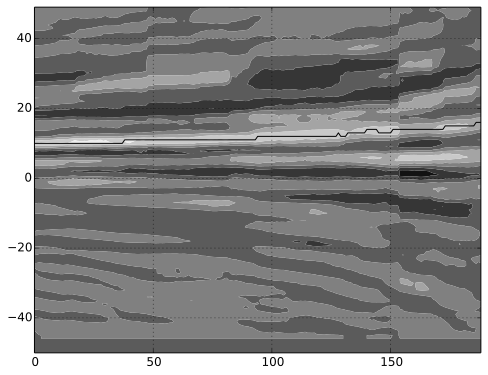
\includegraphics[width=\columnwidth]{selection.pdf}
\caption{Local search strategy for shift selection. The contour map shows shift likelihood across a sequence of shift vectors. Horizontal axis is shift vector index (k), while vertical axis is image shift in columns of width $d$ (p). Brighter points indicate higher likelihood. Values at $p_0 = 0$ indicate the likelihood of no shift, values at $p_l > 0$ indicates likelihood of left shift by $p_l$ columns, and $p_r < 0$, of right shift by $|p_r|$ columns. Starting from a global maximum estimate, hill climbing is performed to update the selected shift while avoiding too much of a deviation from previous values.}
\label{fig:selection}
\end{figure}

After summing the padded and shifted cross-correlation vectors, the resulting \textit{shift vector} (Fig.~\ref{fig:slide_cc}e) is a map of shift likelihoods: the central value indicates the likelihood that no shift has taken place, while values prior to it represent the likelihood of a shift to the left, and values following, of a shift to the right.

All that is left is to select a definite output from the shift vector. It's possible to simply select the position of maximum coefficient at every turn, but this might result in shift estimates changing abruptly over time. A smoother alternative is to select a initial shift estimate, then perform iterative hill climbing over successive shift vectors. Figure~\ref{fig:selection} illustrates the concept.

Let's now turn to the problem of selecting a change image from the teach step to match against the current replay change image. First, a proper definition of what means for a change image in the replay step to ``correspond'' to an image in the teach step is required. Given a function $(x, y, \theta) = o(t)$ of the robot's pose, the \textit{frame correspondence} function $c(t_t, t_r, k)$ can be defined as:
\begin{equation}
c(t_t, t_r, k) = \arg \min_{k' \in [1, n]} {\| o(p(t_t, k')) - o(p(t_r, k)) \|}
\end{equation}

That is, change image $DiVS(w, t_t, k')$ in the range $[DiVS(w, t_t, 1), \dotsc, D(w, t_t, n)]$ ``corresponds'' to current change image $DiVS(w, t_r, k)$ if $k'$ is such that it minimizes the norm of the difference $\| o(p(t_t, k')) - o(p(t_r, k)) \|$ over the range $[1, n]$. Obviously, if $o(t)$ were reliably known at any time, there would be no need for drift estimation in the first place. Therefore what is required is an approximation to $c(t_t, t_r, k)$ that circumvents this requirement.

Several different strategies can be considered. The trivial solution is to correspond change images by index:
\begin{equation}
c_i(t_t, t_r, k) = k
\end{equation}

This may work reasonably well if the robot is driving at the same, constant speed in both the teach and replay steps, and images are sampled at regular intervals (which might depend on implementation factors, such as hardware resources, or how the underlying operating system schedules processes and handles interruptions).

A slightly more elaborate option is to correspond change images by time of acquisition, relative to the start of the step:
\begin{equation}
c_t(t_t, t_r, k) = \arg \min_{k' \in [1, n]} {| (p(t_t, k') - t_t) - (p(t_r, k) - t_r) |}
\end{equation}

This may work better than the previous option when guarantees on regular sampling are poor, but it still assumes a constant speed shared across the two steps.

It's also possible to correspond change images by the distance $s = d(t_0, t)$ traveled since the start of the step:
\begin{equation}
c_d(t_t, t_r, k) = \arg \min_{k' \in [1, n]} {| d(t_t, p(t_t, k')) - d(t_r, p(t_r, k)) |}
\end{equation}

It may seem contradictory to employ traveled distance on a system ostensibly meant to compensate for inaccuracies in odometry data, but it could work if the origin location is regularly reset -- for example, after the robot passes by key landmarks.

In the implementation and tests detailed later on the distance-based matching strategy is used, but in fact after several tests performed on a range of $10m$ to $20m$, no significant performance difference was found among the three.

Finally, the frame selection function must be defined. The problem is how to ensure that any two subsequent images $(S(p(t, k)), S(p(t, k+1)))$ are different enough to provide useful information, but not too different, as this would increase noise. A simple solution is to again rely on traveled distance, defining  $p(t, k)$ as:
\begin{equation}
p(t, k) = \arg \min_{t'} {(k - 1)q \leq d(t') - d(t)}
\end{equation}

Where $q$ is the minimal distance traveled by the robot between $p(t, k)$ and $p(t, k+1)$.

\section{Control Model}

\begin{figure}[b]
\centering
\includegraphics[width=\columnwidth]{clutter.pdf}
\caption{Effects of following a curved path to the current replay change image. As the robot turns in response to an estimated shift, the initially sparse replay change image (a) becomes cluttered with changing regions that fell out of alignment with the current sequence (b).}
\label{fig:clutter}
\end{figure}

Given an estimated shift between the current replay change image and its correspondent from the teach step, steering towards the direction opposite to the shift should reduce and eventually eliminate it, as the robot returns to the teach path. Empirical tests indicate that image shifts (which are measured in pixels) are numerically close enough to drifts in heading direction (measured in degrees) and sideways distance from the teach path (measured in meters), that the later can be estimated from the former merely by application of a weighting term and cut-off limits. In more precise terms, given a shift estimate $s$ measured in pixels from the center, such that positive values represent shifts to the left and negative values, to the right, the estimates for heading direction drift $\Delta \theta$ and sideways drift $\Delta y$ are defined as:
\begin{equation}
\Delta \theta =
\left\{
\begin{array}{r r}
-10^o & \text{if } s \leq -10 \\
10^o & \text{if } s \geq \;\;\;\, 10 \\
s^o & \text{otherwise}
\end{array}
\right.
\end{equation}
\begin{equation}
\Delta y =
\left\{
\begin{array}{r r}
-0.5m & \text{if } s \leq -50 \\
0.5m & \text{if } s \geq \;\;\;\, 50 \\
\frac{s}{100}m & \text{otherwise}
\end{array}
\right.
\end{equation}

Unfortunately, the task of actually steering the robot in response to estimated drifts is complicated by the effects of curved paths on change images. As Figure~\ref{fig:clutter} shows, the moment the robot starts turning in response to a shift estimate, the changing regions of the visual field fall out of alignment with the ongoing sequence, cluttering the change image. To account for this, every time the robot starts moving in a curved path -- which it will do in order to compensate for a non-zero drift estimate -- it immediately stops collecting images. After movement has stabilized in a new straight path, a new ``time zero'' for change image calculation is set, so any images collected before that moment are ignored. Obviously this implies the robot will ``run blind'' for a time, unable to further estimate shifts until heading direction stabilizes.

\section{Experiments}

A Yamabico robot with a stock web camera mounted to its front was employed in a series of experiments to evaluate the model described above. Its implementation was in the form of the C++ library \textbf{Cight}. Built on top of OpenCV, its source code is available on the web under an Open Source license~\cite{HEL14c}. Runtime profiling shows change image computation under Cight is remarkably fast: after the first $w$ difference images have been calculated, it takes a little over $40,000$ CPU cycles (about $0.04$ seconds in an $2.67GHz$ Intel Core i5 processor) to compute an additional difference image and recalculate the change image.

\begin{figure}[b]
\includegraphics[width=\columnwidth]{environments.pdf}
\caption{Environments used in experiments. (a) View from the front entrance of research building 3L. (b) Parking lot behind the building. (c) Corridor in front of laboratory room 3D402.}
\label{fig:environments}
\end{figure}

\begin{figure}[h!]
\subfloat[Entrance of building 3L]{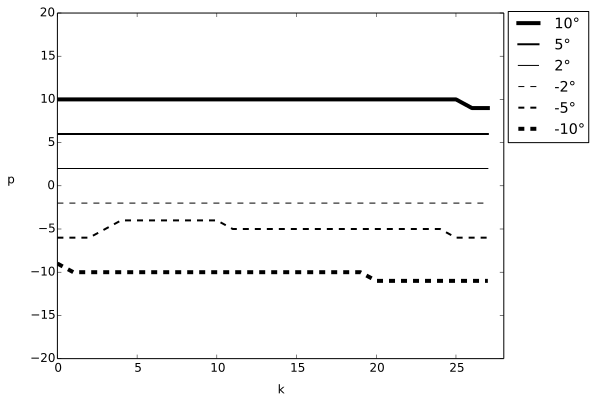
\includegraphics[width=\columnwidth]{entrance_3l_turn.pdf}}\\
\subfloat[Parking lot behind 3L]{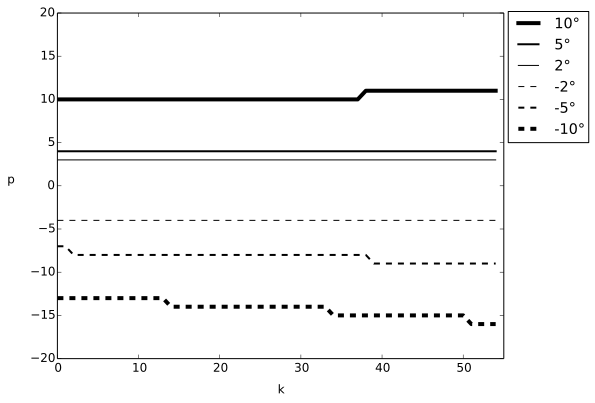
\includegraphics[width=\columnwidth]{car_park_3l_turn.pdf}}\\
\subfloat[Corridor outside room 3D402]{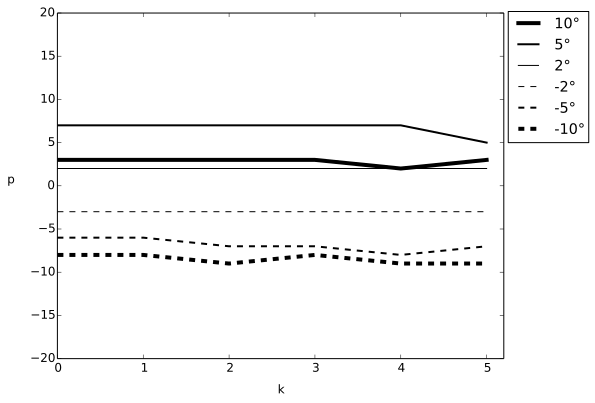
\includegraphics[width=\columnwidth]{corridor_3d_turn.pdf}}
\caption{Shift estimates between teach paths. For each test environment, a reference ``central'' teach path is recorded, as well as six others starting from the same location, but differing by an initial in-place turn of $2^o$, $5^o$ or $10^o$ degrees, either to the left or right. Plots show shift estimates between change images from the reference ``central'' path and each of the ``other'' paths. The horizontal axis refers to change image pairings, and the vertical axis, to the estimated shift. As mentioned previously, positive values across the vertical axis indicate shifts to the left, and negative values, shifts to the right. Sessions recorded in front (a) and behind (b) building 3L, and in the corridor outside of room 3D402 (c). The last two teach steps (with deviations of $10^o$ and $-10^o$) recorded outside room 3D402 were not used, because the corridor was too narrow, and they had to be aborted before the first 25 images could be recorded.}
\label{fig:tests_turn}
\end{figure}

\begin{figure}[h!]
\centering
\includegraphics[width=\columnwidth]{changes.pdf}
\caption{Method robustness to lighting and landscape composition changes. Even though visual input for the teach (a) and replay (b) steps differ substantially, the corresponding change images (c, d) include a number of shared features.}
\label{fig:changes}
\end{figure}

\begin{figure}[h!]
\includegraphics[width=\columnwidth]{pedestrian.pdf}
\caption{Resilience against moving elements. Two teach steps were recorded for the same starting point and heading direction. The first step (a) was recorded in the absence of any moving elements, but in the second (b) a person happened to walk by the robot. Despite this, shift vectors (c) correctly indicate negligible drift was experienced between the steps.}
\label{fig:pedestrian}
\end{figure}

System parameter values $(w = 25, d = 50, e = 5)$ were empirically determined and used throughout all experiments. Three test environments were used, as illustrated in Figure~\ref{fig:environments}: two outdoors (the front entrance and parking lot behind building 3L) and one indoors (the corridor in front of room 3D402). Tests were performed at different times of the day and varying weather conditions. Linear speed was always set to $0.3m/s$, with pictures and odometry recorded every $1.5cm$ on average.

Seven different teach steps were recorded in each environment: a ``central'' recording and six others, deviating from the original by an in-place turn of $2^o$, $5^o$ or $10^o$, either to the left or right. At each session the robot would adjust its heading direction as required, then set off in a straight path for $10m$ or until receiving an abort command (which was sometimes necessary to avoid hitting some obstacle). Figure~\ref{fig:tests_turn} shows results for these tests. The last two teach steps (with deviations of $10^o$ and $-10^o$) recorded outside room 3D402 were not used: because the corridor was too narrow, they had to be aborted before the first 25 images could be recorded.

Some experiments under changing lighting conditions and landscape composition were also performed. Since DiVS shift estimation does not compare individual images, but rather the {\it rates of change} in pairs of image sequences, it is inherently robust to changes that are consistent across whole image sequences, such as overall luminance. It also has a degree of natural resilience to landscape changes, provided they don't substantially affect the rate of change. Figure~\ref{fig:changes} shows an example case.

\begin{figure}[h!]
\includegraphics[width=\columnwidth]{shift_problem.pdf}
\caption{Changes to apparent position of a far-off landmark relative to the robot's field of view. Starting from a position of perfect alignment between the robot's and landmark's centers (a), an in-place turn of as little as $5^o$ produces a large disparity (b); in contrast, the disparity after a sideways displacement as large as half the robot's width is much shorter (c).}
\label{fig:shift_problem}
\end{figure}

\begin{figure}[h!]
\centering
\subfloat[]{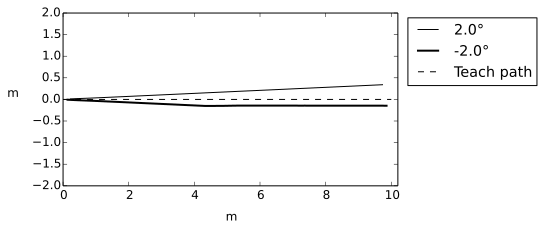
\includegraphics[width=\columnwidth]{steering_2.pdf}}\\
\subfloat[]{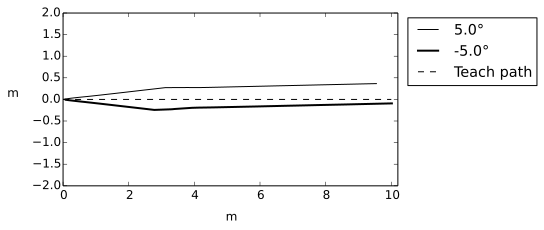
\includegraphics[width=\columnwidth]{steering_5.pdf}}\\
\subfloat[]{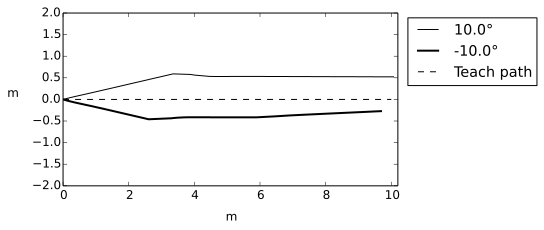
\includegraphics[width=\columnwidth]{steering_10.pdf}}
\caption{Results for replay tests performed before the front entrance of building 3L. Ecah plot shows a teach step path (the dashed line) where the robot ran in a straight line from pose $(x_0, y_0, \theta_0) = (0m, 0m, 0^o)$ to pose $(x_n, y_n, \theta_n) = (10m, 0m, 0^o)$, and two replay paths, with initial left (solid line) and right (solid bold line) in-place turns to simulate drift. Values used for initial in-place turns were $2^o$ (a),  $5^o$ (b) and $10^o$ (c). Horizontal axis corresponds to the $x$ component of robot pose, and vertical axis, to the $y$ component. Heading direction component $\theta$ is not shown but can be inferred by the form of the path lines.}
\label{fig:replay_tests}
\end{figure}

While most recorded teach steps do not depict any moving elements, some unintended records of people walking by the robot were kept for evaluation. Figure~\ref{fig:pedestrian} shows one such case, where despite presence of a walking person in one teach step, but not the other, did not affect the system's correct assessment that there was no significant drift between the teach steps.

Shift estimate failures have two main causes. If input images are too ``plain'', without enough discontinuities, change images become too sparse. This is often compounded by differences in visible objects close to the borders of image sequences, which gain undue importance under these conditions. Moreover, if two image sequences are recorded over paths parallel to it other, it may be very difficult to correctly estimate the shift between the corresponding change images. This is because, as shown in Figure~\ref{fig:shift_problem}, differences in sideways position produce much less disparity in far-off landmarks, which compose the bulk of the landscape in many environments, especially outdoors. This results in much more subtle differences between change images, which are harder to correlate.

After the performance of the shift estimator was properly evaluated off-line, replay steps were also performed. Figure~\ref{fig:replay_tests} shows results of replay step tests performed in front of building 3L, for initial in-place turns of $2^o$, $5^o$ and $10^o$ (both to left and right). In general the robot is able to detect and counteract drifts in heading direction relative to the teach path, but as noticed before, sideways drifts are much harder to infer, sometimes even leading to incorrect estimates.

\section{Conclusion}

This article presented the \textit{Differential Visual Stream} (DiVS) image processing method. It computes a graphical representation of the changes observed in subsequent landscape images captured by an approaching observer. Such change images, when computed from sequences collected at similar positions in the same environment, can be compared in terms of horizontal shift. This in turn can be used to implement appearance-based navigation. Because the change images computed by DiVS attenuate or outright erase many of the transitory differences between images of a same landscape, robust navigation can be achieved against changing environmental conditions.

A number of points still have to be addressed, however. Estimate errors, either due to lack of details in input images or under sideways drift (where the robot is running over a path parallel to the teach path), is the most immediate issue. In fact a more systematic assessment of the method's performance is in order -- in particular, very few tests involving moving elements have been performed. Also required is an analysis of the parameters used across all three stages (change image calculation, shift estimation, steering control) of the system: their values have so far been determined empirically, without a proper understanding of their relative impacts on system performance and relationship to different environmental conditions. The method's current inability to work with curved paths imposes serious limitations on the control model, which in its present form is rudimentary at best, as it can only guide the robot over simple straight paths.

Finally, change image correspondence by traveled distance requires a kind of sensor data (odometry) that is neither always available, nor reliable over long ranges. Correspondence by analysis of the change images themselves, or some other visual method, would be a more portable alternative, enabling the method to work in the absence of any sensor data other than an image stream.

\vfill

\footnotesize

\bibliographystyle{IEEEtran}
\bibliography{references}

\normalsize

\end{document}
